\documentclass{article}
\usepackage[utf8]{inputenc}
\usepackage{multicol}
% maxamize space on paper
\usepackage[nomarginpar, margin=.1in]{geometry}
\usepackage{sectsty}
\usepackage{amsmath}
\usepackage{tikz} 
\sectionfont{\fontsize{9}{9}\selectfont}
\subsectionfont{\fontsize{9}{9}\selectfont}
\subsubsectionfont{\fontsize{9}{9}\selectfont}
\usepackage[compact]{titlesec}
\usepackage{enumitem}
\setlength{\parindent}{0pt} 
\setlist[1]{itemsep=-5pt}
\setlist[2]{itemsep=-5pt}
\begin{document}
\underline{This document is currently incomplete - Information may be incorrect - Please contribute on GitHub!}

\section{P, NP, NP-Completness}

\underline{P:} Generally refers to problems that can be solved in polynomial time

\underline{NP:} Generally refers to problems that can have their solution verified in polynomial time

\underline{NP-Complete:} A problem in NP in which a polynomial-time algorithm that can reduce
the it into any other NP-Complete problem. 

\underline{NP-Hard:} A set of problems that are hard to solve and verify, with some problems not being decideable. Reducable to any problem in NP

\underline{P vs NP:} The P vs NP problem is an unsolved problem on wether a problem whose solution can be
verified in polynomial time can also be solved in polynomial time. 

\underline{Proving NP-X via reduction:} If we wanted to prove that Problem B is NP-X
, we would reduce Problem A (which is known to be NP-X) to it ($A \leq_p B$). 

\section{Graph Coloring}
Given a graph $G = (V, E)$, find the smallest number of different colors to assign for 
each nod ein $G$ so that no two nodes of the same color share an edge. Decision version: 
Given a graph $G$ and a bound $k$, does $G$ have k-coloring?

Simple when $k=2$ since you just need to check if $G$ is bipartite

When $k=3$, we must prove that it is NP-Complete by reducing it to 3-SAT (2-SAT $\leq_p$ 3-Coloring)

\section{Hamiltonian}
\subsection{Hamiltonian Cycle (NP-Hard)}
Does a graph $G = (V, E)$ have a cycle $P$ such that for all $v$ in $V$, $v \in P$?

\subsection{Hamiltonian Path (NP-Hard)}
Does a graph $G = (V, E)$ have a path $P$ such that for all $v$ in $V$, $v \in P$?
Typically when reducing a problem to hamiltonian path, we want to add 2 extra verticies denoting
where we want the path to start and end. If we wanted to test if there is a hamiltonian path from 
$v_0$ to $v_5$, then we would create nodes $s$ and $t$ and create edges $(s, v_0)$ and $(v_5, t)$
and then check if a path from $s$ to $t$ exists.

\section{Approximation}
\underline{Linear Programming:} Given a set of inequalities that represent constraints, our
goal is to minimize or maxamize a certain quantity represented 
by an equation.

$N<1$-approximations is typically used to represent maxamization problems while
an $N>1$-approximation is typically used to represent a minimization problem. 
$N$-approximation means that the solution is within $OPT*N$

In order to do this, find the worst case and then find a way to relate it to the best case.
A good way to do this is to try to think of inputs that would be really bad for the algorithm
and then try to deduce why it may be bad

\subsection{Load Balancing (Search: NP-Hard, Decision: NP-Complete)}
This problem is an example for an approx. algirhthm. Given $M$ machines $m_1, m_2, ..., m_n$ and $n$ jobs where each job $j$ has a processing time
$t_j$, assign each job to a machine and balance the loads across all machines.

\subsection{Vertex Cover (Search: NP-Hard, Decision: NP-Complete))}
The vertex cover problem is a problem in which you want to find a set $S$ of verticies in a graph such that
every edge connects to one of the verticies in $S$.

\subsection{Set Cover (Search: NP-Hard, Decision: NP-Complete)}
The set cover problem is a problem in which you are given a set $M$ of sets and a set $U$ of numbers. Your
goall is to find a union of some sets in $M$ such that their union equals $U$

\section{PSPACE and PSPACE-Completeness}
PSPACE is the set of decision problems that can be solved by a Turing Machine with a polynomial amount of
space. 

PSPACE-Completeness refers to a PSPACE problem in which every other PSPACE problem could be transformed to it in 
polynomial time

\section{Turing Machines}
A turing machine is an abstract machine that given enough time and space can solve any problem. It
is typically represented as a list of cells that has a head which moves to a certain cell, reads a value
and then depending on it's state, usually denoted by $q_n$, it decides what to write to the current cell,
and where to move the head next. The list of states and their outputs can be represented as a series of functions, 
or it can be represented visually as a FSM (Finite State Machine) where each state has a vertex on a graph, and the
possible actions based on the value of the current cell is represented as an edge that specifies direction and then 
some next state. We can represent the state of a turing machine as a list of the cells, with the head at the position
before the cell it is currently reading. The head will be represented by a symbol which represents the current state.

\begin{multicols}{2}
    

For example, these plain english instructions:

State $q_0$:

If cell has value $a$ then go to state $q_0$ and set cell to $b$ and do not move head.

If cell has value $b$ then go to state $q_1$ and move to the right one cell.

State $q_1$:

If cell has value $b$ then go to state $q_0$ and set cell to $a$

If cell has no value ($\sqcup$) then go to state $q_1$ and set the cell to $a$

If cell has value $a$ then go to state $q_{accept}$ (i.e. HALT)

\columnbreak

Can be represented by the functions:


$\delta(q_0, a)  = (q_0, b, /)$

$\delta(q_0, b)  = (q_1, /, R)$

$\delta(q_1, b)  = (q_0, a, /)$

$\delta(q_1, \sqcup)  = (q_1, a, /)$

$\delta(q_1, a)  = (q_accept, /, /)$

\end{multicols}

This can also be represented by the following FSM:

\begin{multicols}{2}
    

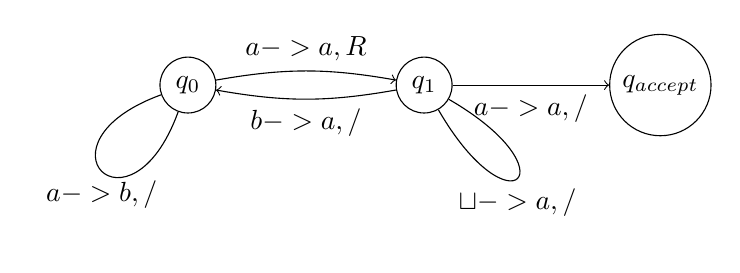
\begin{tikzpicture}[node distance={30mm}, main/.style = {draw, circle}] 
    \node[main] (0)  {$q_0$};
    \node[main] (1) [right of=0] {$q_1$};
    \node[main] (2)  [right of=1] {$q_{accept}$};

    \path [->,bend left=10] (0) edge node [above] {$a -> a, R$} (1);
    \path [->,bend left=10] (1) edge node [below] {$b -> a, /$} (0);
    \path (1) edge [out=330,in=300,looseness=25] node[below] {$\sqcup -> a, /$} (1);
    \path (0) edge [out=200,in=250,looseness=15] node[below] {$a -> b, /$} (0);
    \path [->] (1) edge node [below] {$a -> a, /$} (2);
\end{tikzpicture}

\columnbreak

So a machine in the state $q_0 a \sqcup\sqcup$ would transition through the following states:

$q_0 a \sqcup\sqcup$

$q_0 b \sqcup\sqcup$

$a q_1 a\sqcup$

$a q_{accept} a\sqcup$

\end{multicols}

\section{Undecidability and Halting problem}
An undecidable problem is a problem in which no algorithm can produce a correct response on every
input. In order to prove a problem is undecidable, we can reduce another undecidable problem to it, 
or we can use a proof by contradiction by specifying a scenario in which it wouldn't be possible
to return a correct result (how the Halting problem is commonly proved).

The halting problem is an undecidable problem that takes a function and some input as input. It then returns
wether this program will run forever or if it will eventually halt. It is undecidable because a theoretical
function $C(X) -> if H(X,X) == 'HALT' then LOOP else HALT$ would generate an incorrect output if $C(C)$ is called.


\section{Randomized Algorithms}
Expectance is equal to a value multiplied by the chance that that that value will occur
(this is the average value taken by a random variable)$E(x) = \sum XP(X)$

\subsection{Randomized Median Finding Runtime}
Given an unsorted list $L$, we want to find the median value of that list. To do this, 
we can create an algorithm where we choose a \underline{splitter} $s$, then put every element
larger than $s$ into $S+$ and every element less than $s$ into $S-$. Then, if  $|S-|$ is
equal to $\frac{L}{2}-1$, then $s$ is the median. If $|S-| \geq \frac{L}{2}-1$, then we will
recursively call our function on $|S-|$, else, we eill recursively call our function on $S+$. 

Choosing the splitter can havae major effects on the runtime of the algorithm.

We could choose the splittern in a deterministic way by choosing the first element in the list.

Another (non-deterministic) approach is to choose a number in the list uniformly at random. 

The running time of the algorithm will depend on luck of choosing our splitter. In the worst case, 
It will be $O(n^2)$ if we repedeatly choose the largest element in $L$, since the smallest element
will be in $|S-|$ and each iteration $|S-|$ will be one element smaller than it was last call: $T(n) \leq T(n-1) + c.n$
where $n = |L|$

We know that the randomized algorithm has the possibility of producing outputs such that it would
result in a worse-case runtime, but the probability that it will is much lower. To formalize this:

$T(n)$, the running time of our algorithm on an input of size $n$, is a random variable as it relies 
upon the choice of our random splitter. The algorithm will then split our problem into 2 subproblems that
will have sizes $j-1$ and $n-j$. When choosing how to write our recurrence, we will take the \underline{maximum}
of these 2 as we don't know if the answer will be in $S+$ or $S-$. We can now write our recurrence as:

$T(n) = T(max\{j-1, n-j\}) + O(n)$

We can't solve this as there is an unknown value of $j$ in the recurrence. However we can break this into cases
by using an \textbf{indicator random variable}.

We will decind $X_j$ as the indicator for choosing the $j^{th}$ smallest element from $L$ as the splitter
where $j = 1..n$. No matter what our splitter chooses, exactly one of our indicator variables will be $1$, 
and the rest will be $0$.

Based on $j$, each time we split, one partition will be true. We can base the running time of the algorithm
based on the partitioning cases:

\begin{equation}
    T(n) = 
    \left\{
        \begin{array}{lr}
            T(max\{0, n-1\})+O(n)& \text{if } 0: (n-1) split\\
            T(max\{1, n-2\})+O(n)& \text{if } 1: (n-2) split \\
            ... & ... \\
            T(max\{n-1, 0\})+O(n)& \text{if } n-1: 0 split \\
        \end{array}
    \right\} 
\end{equation}

We can represent $T(n)$ as the summation of every case multiplied by its decision variable (of wich, only one 
will be $1$ and the rest will be $0$)

$T(n) = \sum{j=1}^{n}(X_j(T(max\{j-1, n-j\}) + O(n)))$

We then want to calculate the expectation of $T(n)$, which through a bunch of fancy algebra that
I don't have space for results in:

$\frac{1}{4}c.n - O(N)$ where $c \geq 4 *$ constant of $O$

\section{Misc}



\end{document}
